\documentclass[10pt,a4paper]{article}
\usepackage[margin=2cm]{geometry}
\usepackage{amsmath,amssymb,booktabs,graphicx,caption,subcaption,xcolor,float,hyperref,tikz}
\usetikzlibrary{arrows.meta,positioning,calc}
\hypersetup{colorlinks=true,linkcolor=blue!50!black,urlcolor=blue!50!black}
\captionsetup{font=small,labelfont=bf}
\newcounter{diagram}
\newcommand{\diagramcaption}[1]{\refstepcounter{diagram}\par\smallskip\noindent{\small\textbf{Diagram~\thediagram.} #1}}
\title{\vspace{-1.2cm}\textbf{Tipping an undecided swarm}\\[2pt]
\large Simulation 1, setup \texttt{task003-nosolution}: first results}
\author{LLM-free simulator; extended with the efficiency of control, 12 October 2026; runs of 7 October 2026}
\date{}
\begin{document}
\maketitle
\vspace{-1cm}

\paragraph{How the simulator works.} The world, \texttt{task\_003}, has three candidate
allocations; A0 is the correct one. Each of 24 agents is given one true fact about it and reasons as
an exact Bayesian: its \emph{belief} is the exact probability of A0, A1 and A2 given the facts it
currently remembers. An episode has 30 rounds, each a day and a night. During the day the agents act
one at a time in a new random order: an agent reads $q$ posts drawn at random from a shared
\emph{board} (never its own), adds their facts to its memory, recomputes its belief, \emph{votes}
(\emph{argmax}: the most probable allocation; \emph{probability matching}: a vote drawn from its
belief) and posts one remembered fact that supports its vote, or nothing if none does. At night a
\emph{controller} with a target, A0 (truth) or A2 (false), reads $q_c$ agent posts; unless at least
75\% of them come from agents voting for its target, or what it read already proves its target, it
posts the $b$ facts from its own pool that best support its target. The board is then cleared,
keeping only the controller's new posts. At each dawn every remembered fact is forgotten with
probability $1-\rho$ and comes back if read again. Every episode is run three times with the same
random draws: without a controller, with the truth controller and with the false controller.

\paragraph{Summary.} 24 agents hold evidence that, pooled, is exactly a coin flip between
allocation A0 (the truth) and A2, with no proof available to anyone. A controller steers
toward A0 or A2 using one shared pool of facts. With agents that vote by
\textbf{probability matching}, the swarm stays undecided on its own, and \textbf{either
controller tips it within a few days}; the truth controller does so more easily. With
\emph{argmax} voting and vote-supporting posts, the swarm instead locks into unanimity by
itself, and a design detail (an expected start of 7 / 6 / 11 votes) makes it drift to A2;
we explain this special case and how to remove it. Two further results come from the
design rather than the swarm: \textbf{a larger posting budget can backfire} because the
pool has few facts per target; and the controller \textbf{senses the swarm accurately}.

\section{Setup}

\begin{center}
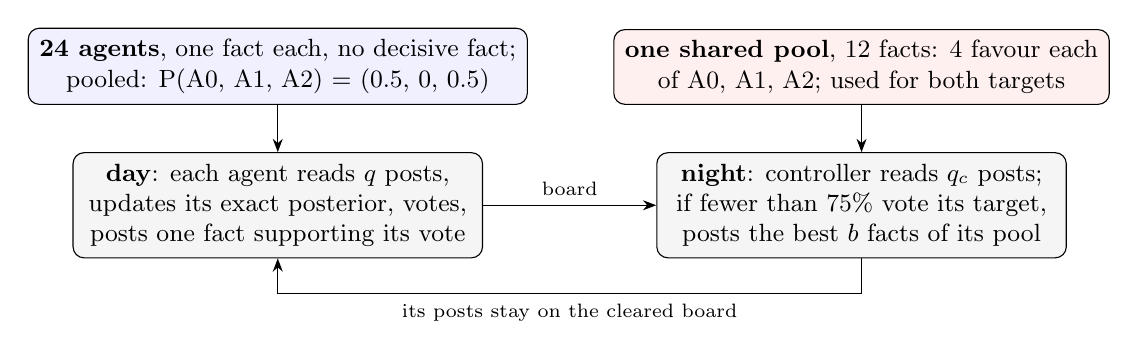
\begin{tikzpicture}[font=\small, box/.style={draw, rounded corners, align=center, inner sep=4pt}]
  \node[box, fill=gray!8, minimum width=5.2cm] (day) {\textbf{day}: each agent reads $q$ posts,\\
     updates its exact posterior, votes,\\ posts one fact supporting its vote};
  \node[box, fill=gray!8, right=2.2cm of day, minimum width=5.2cm] (night) {\textbf{night}: controller reads $q_c$ posts;\\
     if fewer than 75\% vote its target,\\ posts the best $b$ facts of its pool};
  \node[box, fill=blue!6, above=0.6cm of day, minimum width=5.2cm] (agents) {\textbf{24 agents}, one fact each, no decisive fact;\\
     pooled: P(A0, A1, A2) = (0.5, 0, 0.5)};
  \node[box, fill=red!6, above=0.6cm of night, minimum width=5.2cm] (pool) {\textbf{one shared pool}, 12 facts: 4 favour each\\
     of A0, A1, A2; used for both targets};
  \draw[-{Stealth}] (agents) -- (day);
  \draw[-{Stealth}] (pool) -- (night);
  \draw[-{Stealth}] (day) -- node[above, font=\scriptsize]{board} (night);
  \draw[-{Stealth}] (night.south) -- ++(0,-0.45) -| node[below, pos=0.25, font=\scriptsize]{its posts stay on the cleared board} (day.south);
\end{tikzpicture}
\diagramcaption{One round of Simulation 1, repeated for 30 rounds. Each dawn, every
remembered fact survives with probability $\rho$.}
\label{dia:setup}
\end{center}

No proof is available to anyone, not even if the controller posted its whole pool: the
agents' facts plus the whole pool give (0.75, 0, 0.25). The truth keeps an edge that
cannot be designed away (every fact is true): pooled agents plus the best part of the
pool reach at most P(A0) = 0.92, but P(A2) = 0.77.

Agents are exact Bayesian reasoners with posterior $P_j = (P_j(\text{A0}), P_j(\text{A1}), P_j(\text{A2}))$
over the facts they remember. They vote by one of two rules:
\begin{align}
\text{probability matching:}\quad & \Pr(\text{vote}_j = k) = P_j(k), \label{eq:pm}\\
\text{argmax:}\quad & \text{vote}_j = \arg\max_k P_j(k), \text{ ties broken at random.} \label{eq:argmax}
\end{align}
Control is measured by the \emph{paired gain}: each episode is run silent, with the truth
controller, and with the false controller, using the same random draws, and
\begin{equation}\label{eq:gain}
G_t^{(a)} = \frac{1}{E}\sum_{e=1}^{E}\Bigl[x_{a,t}^{\text{ctrl}}(e) - x_{a,t}^{\text{silent}}(e)\Bigr],
\end{equation}
where $x_{a,t}$ is the share of agents voting $a$ on day $t$, $E = 1000$ episodes.

\section{Main result: with probability matching, either controller tips the swarm}

\paragraph{Without a controller the swarm stays undecided.} Under probability matching
no episode ever becomes unanimous, and the A2 $-$ A0 vote margin stays near zero
(Figure~\ref{fig:drift}, red): exactly 0 with full memory, and a small lean of
+0.07 to +0.15 toward A2 when agents forget (A2-side facts survive forgetting better:
held by 53\% of agents on day 30, A0-side facts by 31\%).

\paragraph{With a controller it tips within days.} Figures~\ref{fig:phasetruth}
and~\ref{fig:phasefalse} show the day-30 gain for every reading budget $q_c$ and posting
budget $b$; Figure~\ref{fig:gaintime} shows how the gain builds up over the days.

\begin{table}[H]
\centering\small
\caption{Probability matching, day 30, $q_c = 12$, $b = 3$: paired gain in the target's
share, Eq.~(\ref{eq:gain}), for $q = 3 / 6 / 12$; and the share of episodes in which
the target passes 75\% by day 30 (mean over $q$), with the silent value in brackets.}
\label{tab:pm}
\begin{tabular}{llccc}
\toprule
$\rho$ & controller & gain ($q = 3 / 6 / 12$) & target past 75\% & median day \\
\midrule
0.75 & truth (A0) & 0.33 / 0.42 / 0.43 & 0.99 (0.26) & 3--4 \\
0.75 & false (A2) & 0.21 / 0.25 / 0.23 & 0.98 (0.58) & 3 \\
1.0 & truth (A0) & 0.37 / 0.37 / 0.38 & 1.00 (0.36) & 3 \\
1.0 & false (A2) & 0.08 / 0.07 / 0.06 & 0.90 (0.47) & 3 \\
\bottomrule
\end{tabular}
\end{table}

\begin{figure}[H]
\centering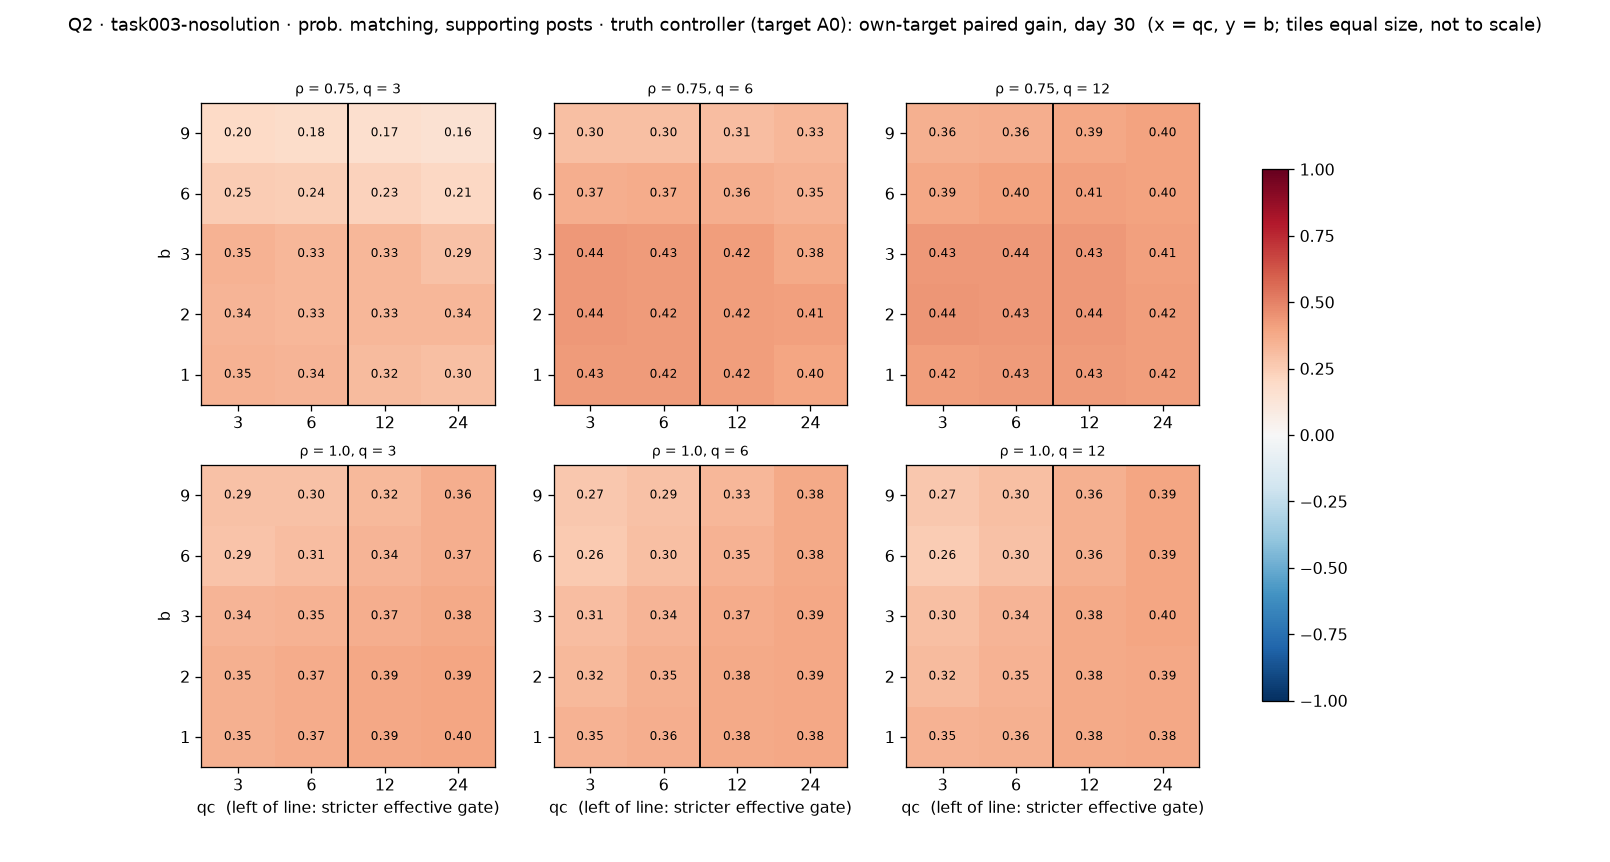
\includegraphics[width=0.9\linewidth]{figures/phase_truth_pm.png}
\caption{Truth controller, probability matching: day-30 paired gain in the A0 share over
$q_c$ (x) and $b$ (y). Rows: $\rho$; columns: $q$. Tiles equal size, not to scale.
Hatched: 95\% interval includes 0. Left of the black line the vote gate is effectively
stricter.}
\label{fig:phasetruth}
\end{figure}

\begin{figure}[H]
\centering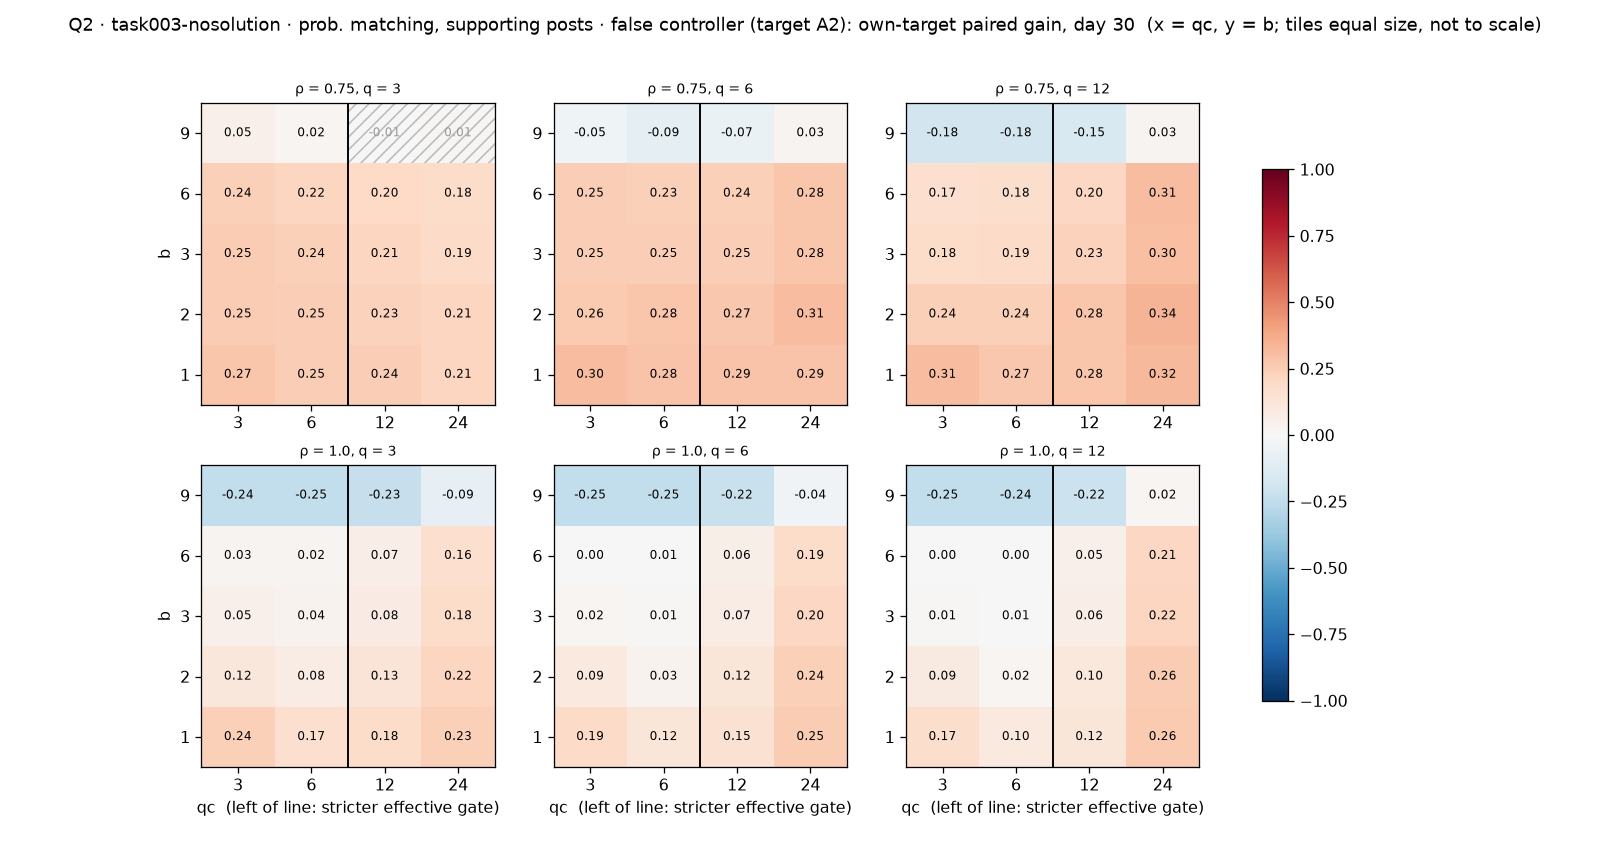
\includegraphics[width=0.9\linewidth]{figures/phase_false_pm.png}
\caption{As Figure~\ref{fig:phasetruth}, for the false controller (gain in the A2 share).}
\label{fig:phasefalse}
\end{figure}

\begin{figure}[H]
\centering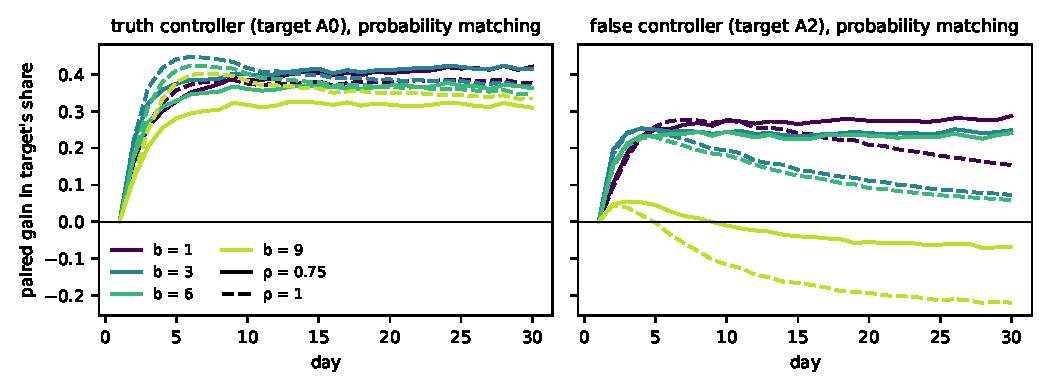
\includegraphics[width=0.95\linewidth]{figures/fig_gain_time.pdf}
\caption{Probability matching: paired gain in the target's share over the days, by
posting budget $b$; $q = 6$, $q_c = 12$. Solid $\rho = 0.75$, dashed $\rho = 1$.}
\label{fig:gaintime}
\end{figure}

\begin{itemize}\itemsep1pt
\item \textbf{Both controllers tip the swarm in about 3 days} (Table~\ref{tab:pm}).
\item \textbf{The truth controller is stronger}, and the gap widens with full memory:
  gains of about 0.37 against 0.07 at $\rho = 1$. As agents accumulate facts, their
  pooled evidence pulls back toward the truth's higher ceiling; the false controller's
  gain decays over the days (Figure~\ref{fig:gaintime}, right, dashed).
\item \textbf{The reading budget $q_c$ matters little}; the posting budget matters only at
  its largest value (Section~\ref{sec:budget}).
\end{itemize}

\section{A special case: the A2 drift under argmax voting}\label{sec:drift}

\begin{figure}[H]
\centering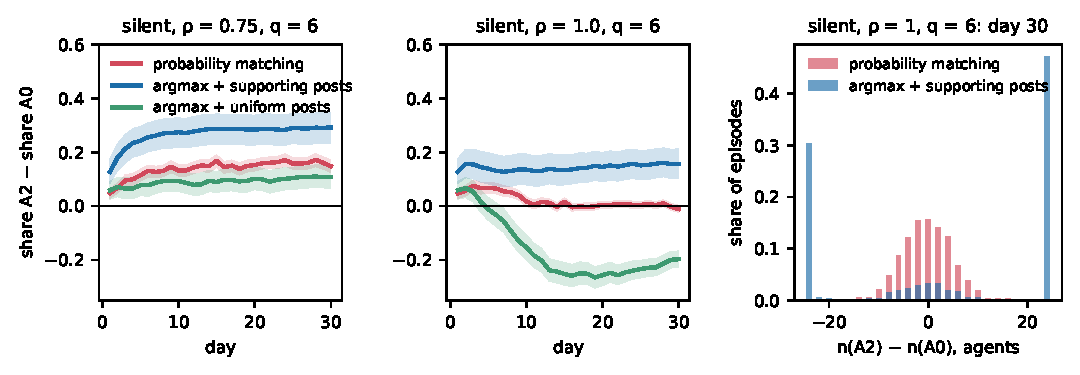
\includegraphics[width=0.98\linewidth]{figures/fig_drift.pdf}
\caption{Silent arm, $q = 6$. Left and middle: A2 $-$ A0 vote margin over the days.
Right: day-30 spread of the margin across episodes, in agents.}
\label{fig:drift}
\end{figure}

With argmax voting and vote-supporting posts (the \emph{base} rule), the silent swarm does
not stay undecided: \textbf{63--91\% of episodes end unanimous}, all 24 agents on A2
(43--67\%) or on A0 (15--41\%). The mean margin toward A2 (Figure~\ref{fig:drift}, blue)
is the difference between those two groups; the histogram shows the lock-in at
$\pm 24$. Three ingredients combine:

\begin{enumerate}\itemsep1pt
\item \textbf{Argmax turns any lead into a vote}, Eq.~(\ref{eq:argmax}).
\item \textbf{Agents post only facts supporting their vote}, so later readers mostly meet
  the majority's evidence, and with forgetting the minority's evidence dies out
  (day 30, $\rho = 0.75$: A2-side facts held by 53\% of agents, A0-side by 24\%).
\item \textbf{The swarm starts with more A2 voters.} Under argmax, an agent holding a fact
  that favours two allocations equally votes for each half the time. Its expected
  starting vote is
  \begin{equation}\label{eq:startvote}
  \mathbb{E}[n_k] = \sum_{j=1}^{24} \frac{\mathbb{1}\{k \in \arg\max P_j\}}{|\arg\max P_j|},
  \end{equation}
  which gives \textbf{7 / 6 / 11} for A0 / A1 / A2 (Table~\ref{tab:start}).
\end{enumerate}
Remove ingredient 1 (probability matching) or 2 (uniform posting: post any remembered
fact) and the lock-in collapses: no unanimous episode at all under probability matching,
9--22\% under uniform posting.

\begin{table}[H]
\centering\small
\caption{Why the start is 7 / 6 / 11. The setup balanced agents by \emph{fact group}
(8 per allocation), assigning a tied fact to the lower-numbered allocation; argmax votes
split ties.}
\label{tab:start}
\begin{tabular}{lccc}
\toprule
 & A0 & A1 & A2 \\
\midrule
agents per fact group (design bookkeeping) & 8 & 8 & 8 \\
\quad of which hold a fact tied A1/A2 (counted as A1) & -- & 6 & -- \\
\quad of which hold a fact tied A0/A1 (counted as A0) & 2 & -- & -- \\
expected starting votes, argmax, Eq.~(\ref{eq:startvote}) & \textbf{7} & \textbf{6} & \textbf{11} \\
expected starting votes, probability matching & 8.3 & 7.4 & 8.3 \\
\bottomrule
\end{tabular}
\end{table}

\paragraph{How to fix the start.} Balance the agents on \emph{expected votes},
Eq.~(\ref{eq:startvote}), instead of on fact groups. Under the current rules this is
impossible: none of the 10,438 coin-flip agent sets the builder can produce has equal
expected A0 and A2 votes. The reason is scarcity: only 3 eligible facts favour A1
alone, so any 5-fact A1 group must include A1/A2-tied facts. Dropping the
fact-group rule and requiring expected votes of exactly 8 / 8 / 8 directly works: a
random search found such agent sets (still a coin flip, all facts eligible), e.g.\ 12
facts each held by 2 agents. A full rebuild would also re-check the pool rules (no
shared facts, no joint proof). This changes the frozen setup, so it is a decision, not
yet applied. Probability matching needs no fix: its start is already balanced.

\section{More budget can be worse: a design effect}\label{sec:budget}

At the largest posting budget the controller's gain falls (Figures~\ref{fig:phasetruth},
\ref{fig:phasefalse}, top row; Figure~\ref{fig:gaintime}, $b = 9$), and the false
controller's can even turn negative ($-0.08$ at $\rho = 0.75$, $-0.22$ at $\rho = 1$,
$q_c = 12$, mean over $q$). The cause is arithmetic, not swarm dynamics. The controller
must post exactly $b$ facts or none, and the shared pool holds only $n_{\text{target}}$
facts on its target's side, so each post contains at least
\begin{equation}\label{eq:counter}
c = \max(0,\; b - n_{\text{target}})
\end{equation}
facts that do not favour its target.

\begin{table}[H]
\centering\small
\caption{Pool composition and what the false controller actually posts (probability
matching, $\rho = 1$, $q = 6$, $q_c = 12$). Tied facts count for both sides.}
\label{tab:budget}
\begin{tabular}{lccc}
\toprule
 & $b = 3$ & $b = 6$ & $b = 9$ \\
\midrule
facts in the pool on the target's side ($n_{\text{target}}$) & \multicolumn{3}{c}{A0: 4, \; A2: 6} \\
posted facts favouring A0 / A1 / A2 & 14 / 23 / 62\% & 12 / 22 / 67\% & \textbf{26} / 23 / 51\% \\
nights the controller posts & 59\% & 63\% & \textbf{93\%} \\
\bottomrule
\end{tabular}
\end{table}

The fall starts exactly where Eq.~(\ref{eq:counter}) becomes positive: at $b = 6$ for the
truth controller ($n = 4$), at $b = 9$ for the false one ($n = 6$). Its counter-evidence
keeps the target's vote share below the gate, so it keeps posting (Table~\ref{tab:budget}),
and the counter-evidence accumulates. The effect replicates with fresh random draws
(a second seed). It disappears if the controller may post \emph{up to} $b$ facts, or never posts
facts against its target; in task003-symmetric, whose pools are entirely on their
target's side, more budget simply helps.

\section{The controller senses the swarm accurately}

Each night the controller estimates the share of agents backing its target from the
$n \le q_c$ agent posts it reads, $\hat v = \frac{1}{n}\sum_i \mathbb{1}\{\text{author of
post } i \text{ voted for the target}\}$, and stays silent when $\hat v \ge 0.75$.

\begin{figure}[H]
\centering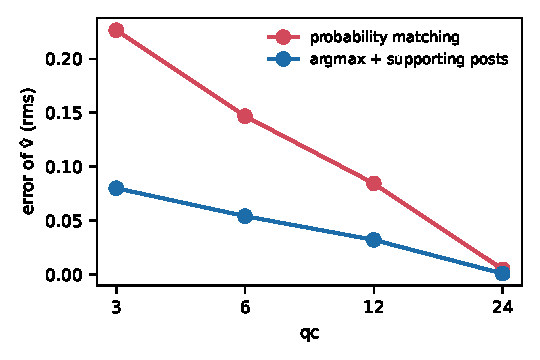
\includegraphics[width=0.45\linewidth]{figures/fig_sensing.pdf}
\caption{Error of $\hat v$ against the true share of all 24 agents, task003-nosolution.}
\label{fig:sensing}
\end{figure}

$\hat v$ is unbiased ($\pm 0.0005$), its error shrinks with $q_c$ and vanishes at
$q_c = 24$ (Figure~\ref{fig:sensing}). It is larger under probability matching because
those swarms stay mixed, which also makes gate mistakes more common: the controller
stays silent although the true share is below 0.75 on 5--8\% of nights, and posts
although it is above 0.75 on up to 13\% at $q_c = 3$. Abstaining agents (0.1--0.2\% of
agent-days) do not bias it.

\paragraph{Helping the truth versus agents' own proofs: does not apply here.} In
task003-symmetric, extra truth posts raise the share of agents holding a proof of A0 but
lower the share holding one from their own evidence. In task003-nosolution no proof is
possible by construction, so this question does not arise.


\section{How efficiently does the controller steer?}\label{sec:eff}

A controller can change the swarm in two ways: in the direction it is asked to, or in ways that
happen whatever its target. We measure how readable the command is in the swarm, how far each
controller gets toward its target, how much of its change is directed, what each fact it posts buys,
and how unsure the agents become. Throughout, the target is chosen by a fair coin, and all
quantities are taken at one time $t$, across the 1{,}000 episodes of each arm (not over whole
trajectories). Setting: probability matching, $q = 6$.

\subsection{Measures}

\begin{center}
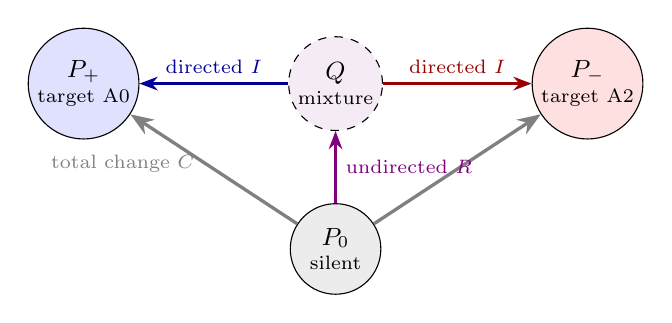
\begin{tikzpicture}[font=\small, dist/.style={draw, circle, minimum size=1.15cm, align=center, inner sep=1pt}]
  \node[dist, fill=gray!15] (P0) at (0,0) {$P_0$\\[-2pt]{\scriptsize silent}};
  \node[dist, fill=blue!12] (Pp) at (-3.2,2.1) {$P_+$\\[-2pt]{\scriptsize target A0}};
  \node[dist, fill=red!12] (Pm) at (3.2,2.1) {$P_-$\\[-2pt]{\scriptsize target A2}};
  \node[dist, dashed, fill=violet!8] (Q) at (0,2.1) {$Q$\\[-2pt]{\scriptsize mixture}};
  \draw[-{Stealth}, very thick, gray] (P0) -- node[left, font=\scriptsize, pos=0.55]{total change $C$} (Pp);
  \draw[-{Stealth}, very thick, gray] (P0) -- (Pm);
  \draw[-{Stealth}, thick, violet] (P0) -- node[right, font=\scriptsize]{undirected $R$} (Q);
  \draw[-{Stealth}, thick, blue!60!black] (Q) -- node[above, font=\scriptsize]{directed $I$} (Pp);
  \draw[-{Stealth}, thick, red!60!black] (Q) -- node[above, font=\scriptsize]{directed $I$} (Pm);
\end{tikzpicture}
\diagramcaption{Three distributions of the swarm's state at time $t$, one per arm, each over the
episodes of that arm. The controller's total change $C$ splits exactly into a part that depends on
its target ($I$, from the mixture $Q$ to each arm) and a part that does not ($R$, from silence to
$Q$). Efficiency $\eta = I/C$ is the directed share.}
\end{center}

\noindent\textbf{Distributions.} For each arm $a$ (silent $0$, target A0 $+$, target A2 $-$) and a
time $t$, each episode $e$ contributes a probability vector $y_a(e)$ over the values $x$ of the
state $X$: at \emph{one-agent} level its vote shares (the vote of a randomly chosen agent), at
\emph{swarm} level a mark on the bin of $s = m_{\text{A0}} - m_{\text{A2}}$ (difference of mean
beliefs, three equal bins on $[-1,1]$). Then $\hat P_a = \frac1n\sum_e y_a(e)$. Any pair of controllers
can be written as
\begin{equation}\label{eq:split}
\hat P_\pm = \hat P_0 + \mu \pm \delta,\qquad \mu = \tfrac12(\hat P_+ + \hat P_-) - \hat P_0,\quad
\delta = \tfrac12(\hat P_+ - \hat P_-),
\end{equation}
a \emph{common} part $\mu$ (what control does on average, whatever the target) and a
\emph{directional} part $\delta$; both are vectors over the values of $X$ (all answers, A1 included).

\noindent\textbf{Readability and the pair efficiency.} With $\hat Q = \hat P_0 + \mu$ and
$\mathrm{KL}(p\Vert q) = \sum_x p(x)\log_2[p(x)/q(x)]$,
\begin{equation}\label{eq:eta}
I = \tfrac12\mathrm{KL}(\hat P_+\Vert\hat Q) + \tfrac12\mathrm{KL}(\hat P_-\Vert\hat Q),\quad
C = \tfrac12\mathrm{KL}(\hat P_+\Vert\hat P_0) + \tfrac12\mathrm{KL}(\hat P_-\Vert\hat P_0) = I + R,\quad
R = \mathrm{KL}(\hat Q\Vert\hat P_0),\quad \eta = I/C .
\end{equation}
$I$ is the mutual information between the target and the state: how readable the command is
(at most 1 bit). $I = \frac12\mathrm{KL}(\hat Q+\delta\Vert\hat Q) + \frac12\mathrm{KL}(\hat Q-\delta\Vert\hat Q)$
depends on $\delta$ and on where the pair sits ($\hat Q$); $R = \mathrm{KL}(\hat P_0+\mu\Vert\hat P_0)$ depends
only on $\mu$; $C$ (a number) $= I + R$, so $R = C - I$. The reference $\hat P_0$ is the silent arm. For
small changes, $\mathrm{KL}(p+\epsilon\Vert p) \approx \sum_x \epsilon(x)^2/(2\ln 2\,p(x))$ gives
\begin{equation}\label{eq:etasmall}
I \approx \frac{\Vert\delta\Vert^2}{2\ln 2},\quad R \approx \frac{\Vert\mu\Vert^2}{2\ln 2},\quad
\eta \approx \frac{1}{1 + \Vert \mu\Vert^2/\Vert\delta\Vert^2},\qquad \Vert v\Vert^2 = \sum_x \frac{v(x)^2}{\hat P_0(x)} .
\end{equation}
So $\eta = 1$ exactly when the two controllers' changes are mirror images ($\mu = 0$), whatever their
size, and $\eta$ falls only through the \emph{ratio} of common to directional change: when both push
the same way (a common push), or one moves the swarm much more than the other (a lopsided pair:
along one direction with sizes $a$ and $b$, $\Vert \mu\Vert/\Vert\delta\Vert = |a-b|/(a+b)$). It is a
property of the pair, not of either controller, and it stays constant whenever both effects grow
together. At swarm level $C$ is often infinite (the controlled swarm reaches states silence never
visits); there we use $\eta_{JS} = I/(I + \mathrm{JS}(\hat Q,\hat P_0))$ with the bounded
Jensen--Shannon divergence; $\mathrm{JS}(\hat Q,\hat P_0)$ is the information the state carries about
\emph{whether} a controller is present (controlled or silent, 50/50), so $\eta_{JS}$ compares
information about the direction with information about the presence of control.

\noindent\textbf{Each controller against its own target} $z$ (one agent, votes):
\begin{equation}\label{eq:progress}
S_z = \mathrm{KL}\big(\mathrm{Bern}(\hat P_z(z))\,\Vert\,\mathrm{Bern}(\hat P_0(z))\big),\qquad
\pi_z = \frac{S_z}{\log_2[1/\hat P_0(z)]},\qquad
\varphi_z = \frac{S_z}{\mathrm{KL}(\hat P_z\Vert\hat P_0)},\qquad
\text{price} = \frac{S_z}{\text{facts posted}} .
\end{equation}
$S_z$ is the least information any intervention must inject to raise the target's share from its
silent value to the observed one (raise the target, scale the other answers in proportion).
\textbf{Progress} $\pi_z$ is the share of the way from silence to unanimity on the target, in bits;
\textbf{focus} $\varphi_z$ the share of the controller's actual change that was needed for that gain;
both are negative when the controller moved its target \emph{down}. The \textbf{price} is the
information injected per fact the controller posted. Finally, the agents' own uncertainty:
$\Delta\bar H$ (mean entropy of their beliefs) and $\Delta$JSD (disagreement, the entropy of the mean
belief minus $\bar H$), controlled minus silent, same episode.

\subsection{Over time, at one setting}

\begin{figure}[!htb]
\centering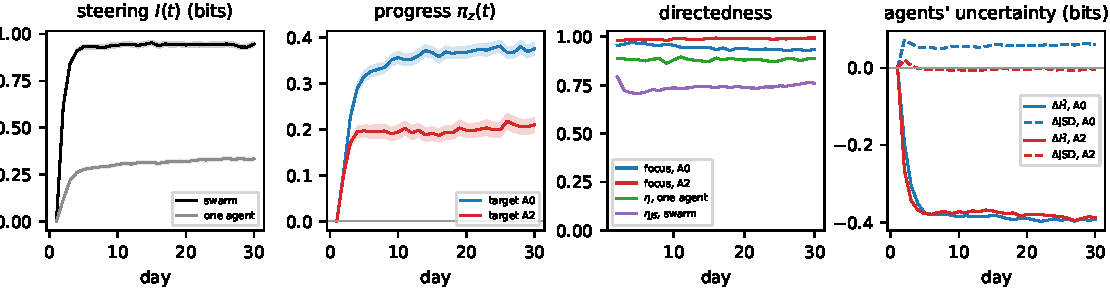
\includegraphics[width=0.92\linewidth]{figures/fig_eff_time2.pdf}
\caption{At $\rho = 0.75$, $q_c = 12$, $b = 3$ (end of each day): readability $I(t)$, each controller's progress $\pi_z(t)$, directedness
(focus $\varphi_z$, pair efficiency $\eta$, $\eta_{JS}$), and the agents' uncertainty. Bands: 95\%
intervals over episodes.}
\label{fig:efftime2}
\end{figure}

\begin{itemize}\itemsep1pt
\item \textbf{Control is reached fast}: 90\% of the day-30 progress by day 9 (target A0) and day 4
  (target A2); $\pi_{\text{A0}} = 0.37$, $\pi_{\text{A2}} = 0.21$ at day 30, with focus 0.93 and 0.99.
\item \textbf{Both controllers make agents surer} ($\Delta\bar H \approx -0.39$ bits); the truth
  controller also splits them a little ($\Delta$JSD $+0.06$).
\end{itemize}

\subsection{Across the control plane}

\begin{figure}[!htb]
\centering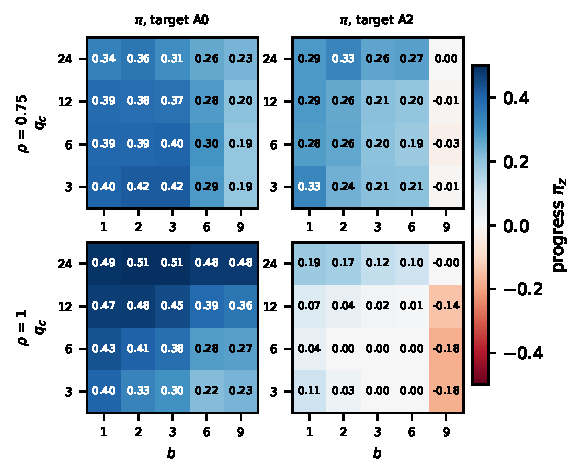
\includegraphics[width=0.44\linewidth]{figures/fig_eff_phase_progress.pdf}
\caption{Progress $\pi_z$ of each controller at $t = 30$ over the reading budget $q_c$ and the facts per night $b$
(one agent, votes). Red: the controller moved its target down. Dash: undefined (silence already at
unanimity).}
\label{fig:effprog}
\end{figure}

\begin{figure}[!htb]
\centering
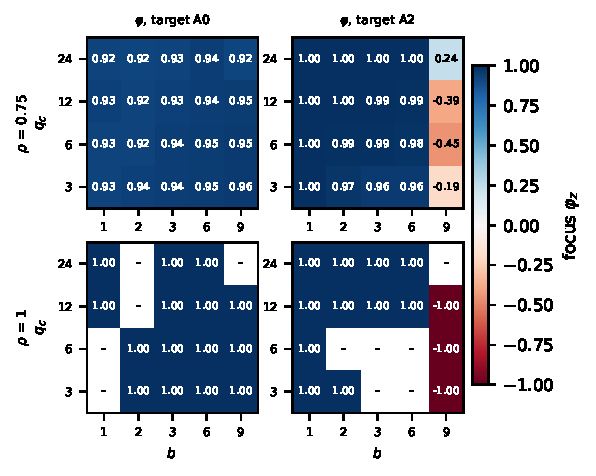
\includegraphics[width=0.38\linewidth]{figures/fig_eff_phase_focus.pdf}\hfill
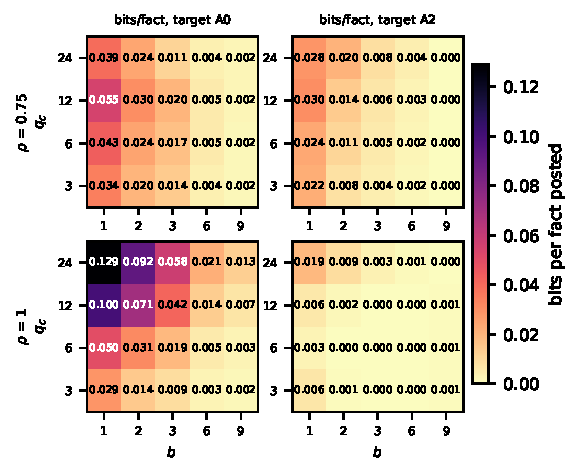
\includegraphics[width=0.38\linewidth]{figures/fig_eff_phase_price.pdf}
\caption{Left: focus $\varphi_z$ (negative: the change went against the target). Right: price,
information injected per fact posted (bits). $t = 30$;  Dash: undefined (no change, or the
controlled swarm considers an answer silence rules out completely).}
\label{fig:efffocusprice}
\end{figure}

\begin{figure}[!htb]
\centering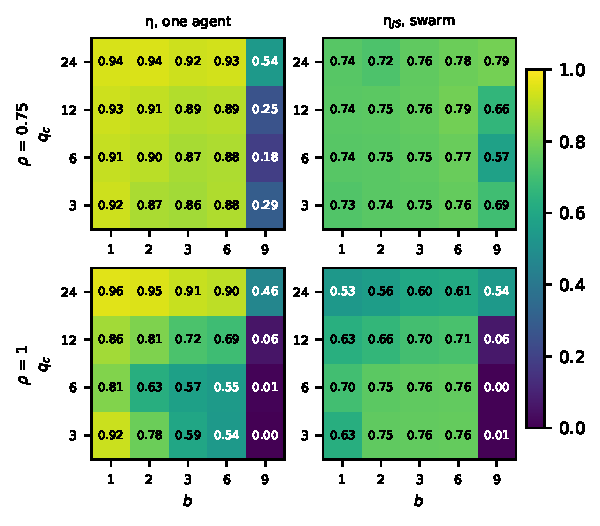
\includegraphics[width=0.36\linewidth]{figures/fig_eff_phase.pdf}
\caption{Pair efficiency at $t = 30$ over $q_c$ and the facts per night $b$: one-agent $\eta$ (beliefs) and swarm
$\eta_{JS}$. Dash: undefined.}
\label{fig:effphase}
\end{figure}

\begin{itemize}\itemsep1pt
\item \textbf{The large-budget backfire is negative progress.} At $b = 9$ the false controller moves
  A2 \emph{down} ($\pi_{\text{A2}}$ down to $-0.03$ at $\rho = 0.75$ and $-0.18$ at $\rho = 1$) and its focus
  turns negative ($-0.19$ to $-0.45$ at $q_c \le 12$; $-1$ with full memory): its change goes against
  its own target.
  The truth controller keeps progressing (0.19--0.51).
\item \textbf{The cheapest control is one fact per night}: the price (target A0) falls from
  0.03--0.13 bits per fact at $b = 1$ to 0.002--0.013 at $b = 9$; with full memory, reading more posts
  makes each fact worth more (0.03 at $q_c = 3$, 0.13 at $q_c = 24$, $b = 1$).
\end{itemize}

\subsection{Readability, pair efficiency and uncertainty against the facts per night}

\begin{figure}[!htb]
\centering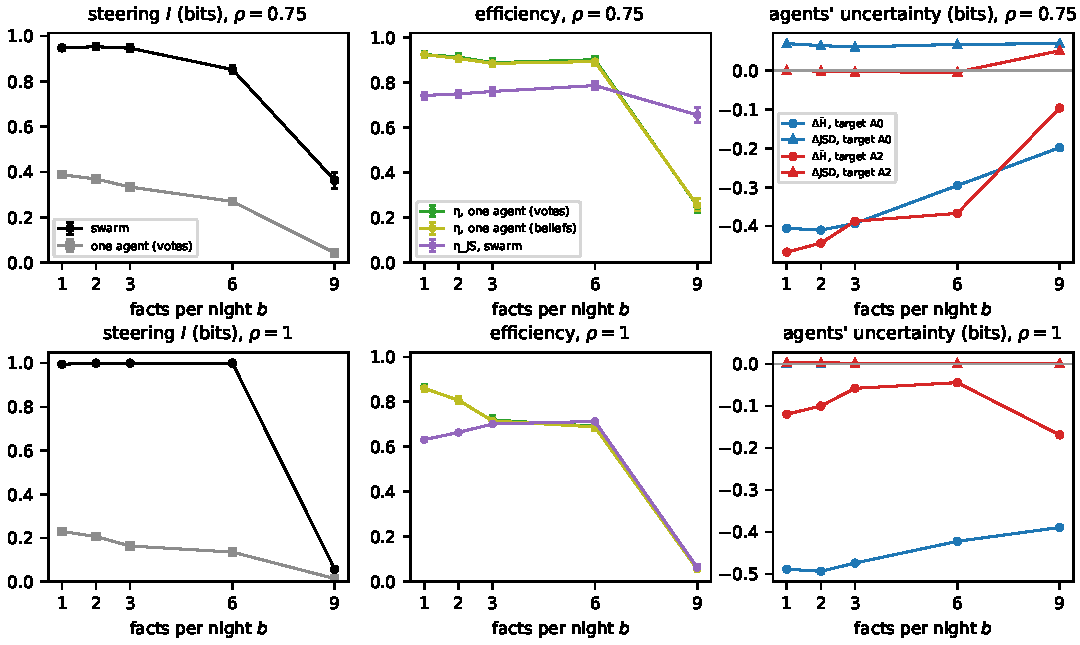
\includegraphics[width=0.72\linewidth]{figures/fig_eff_settings.pdf}
\caption{Readability $I$ (left), pair efficiency (middle) and the change in the agents' uncertainty
(right; circles $\Delta\bar H$, triangles $\Delta$JSD) at $t = 30$ against facts per night $b$ ($q_c = 12$). Bars: 95\% intervals.}
\label{fig:effsettings}
\end{figure}

\begin{itemize}\itemsep1pt
\item \textbf{$\eta$ collapses at $b = 9$} (0.25 at $\rho = 0.75$, 0.06 at $\rho = 1$) through a
  \emph{common push}: both controllers raise A0. Up to $b = 6$, at $\rho = 0.75$, the pair is balanced
  ($\eta \approx 0.9$).
\item The swarm-level readability saturates near 1 bit with full memory (every episode ends on its
  controller's side), so it measures distinguishability, not size; progress measures size.
\end{itemize}

\subsection{Precision at 50, 100 and 300 paths}

\begin{table}[H]
\centering\small
\caption{Value from 1{,}000 paths per arm, and root-mean-square error of the estimate from 50, 100
or 300 paths (200 random subsets each), at $t = 30$, $b = 3$, $q_c = 12$, $\rho = 0.75$. $^\ast$: share of subsets in which
the quantity is infinite or undefined.}
\label{tab:effprec}
\begin{tabular}{lcccc}
\toprule
quantity & 1{,}000 paths & error, 50 & error, 100 & error, 300 \\
\midrule
steering $I$, swarm (3 bins) & 0.946 & 0.034 & 0.024 & 0.012 \\
steering $I$, one agent (votes) & 0.333 & 0.027 & 0.019 & 0.009 \\
efficiency $\eta$, one agent (votes) & 0.889 & 0.038 & 0.027 & 0.013 \\
efficiency $\eta_{JS}$, swarm & 0.761 & 0.038 & 0.025 & 0.013 \\
progress $\pi$, target A0 (votes) & 0.375 & 0.034 & 0.020 & 0.010 \\
progress $\pi$, target A2 (votes) & 0.209 & 0.037 & 0.027 & 0.013 \\
focus $\varphi$, target A0 (votes) & 0.935 & 0.025 & 0.019 & 0.009 \\
focus $\varphi$, target A2 (votes) & 0.994 & 0.014 & 0.008 & 0.004 \\
$\Delta\bar H$, target A0 & -0.393 & 0.036 & 0.026 & 0.012 \\
$\Delta\bar H$, target A2 & -0.387 & 0.034 & 0.025 & 0.012 \\
$\Delta$JSD, target A0 & 0.061 & 0.010 & 0.006 & 0.004 \\
$\Delta$JSD, target A2 & -0.003 & 0.009 & 0.006 & 0.003 \\
\bottomrule
\end{tabular}
\end{table}

\noindent Across all settings, at 100 paths: readability $\pm0.01$ (one agent) to $\pm0.03$ (swarm),
progress $\pm0.02$, focus $\pm0.01$--$0.02$, $\eta$ $\pm0.02$--$0.03$, $\Delta\bar H$ $\pm0.02$, $\Delta$JSD
$\pm0.006$. Two settings that differ by at least 0.02 are ordered correctly in 90--100\% of subsets.

\paragraph{Caveats.} One world (task\_003), 24 agents, exact-Bayesian agents; means over
1,000 episodes per cell. Full analysis, code and tables:
\texttt{analysis/task003\_llm\_free/sim1\_analysis/} (reports Q0--Q6).

\end{document}
